\section{哨兵高分遥感影像超分数据集构建}

\subsection{综述(暂时)}

深度学习超分辨率数据集本质上为一定数量相同场景的高分辨率低分辨率图像对. 现阶段, 用相机拍摄近景的自然影像超分数据集比较成熟, 数量较多. 根据其低分辨率图像获取方法, 主要分为两大类, 第一类如DIV2K~\cite{DIV2K}, BSDS500~\cite{BSDS500}, Set5~\cite{Set5}, Set14~\cite{Set14}, Urban100~\cite{Urban100}等人造低分辨率超分数据集, 这些数据集只含有高分辨率图像, 在进行训练之前, 需要通过先验的图像退化模型进行下采样生成所对应的低分辨率图像, 和原始的高分辨率图像组合成图像对. 在以上自然影像超分数据集制作过程中, 使用的是较为经典的退化模型~\cite{classicDM}, 一般对高分辨率图像进行模糊化(Blur), 噪声模拟(Noise), 下采样(Downsample)后得到低分辨率图像. 然而真实世界的退化模型十分复杂, 经典退化模型过于简单, 无法胜任模拟现实中高分辨率到低分辨率图像的退化过程的任务. 因此, Yuan等人~\cite{CinCycleGAN}, Fritsche等人~\cite{DSGAN}, Wang等人~\cite{DASR}, 构建数据集时, 使用对抗生成网络(Generative Adversarial Networks, GAN~\cite{GAN})学习低分辨率图像的数据分布来得到退化模型, 但通过此种方法训练出的退化模型受限制于其训练数据集数据分布, 如果实际数据分布不同于训练集数据分布, 其训练出退化模型效果不佳. 无论经典退化模型或是训练出的退化模型, 由于模拟生成的低分辨率数据和真实的低分辨率数据在特征空间中总是存在明显差异, 数据鸿沟现象无法避免, 因此往往通过人造低分辨率图像训练得到的模型在现实应用场景效果大打折扣~\cite{SupER}.

与之相对应, 第二类构建超分辨率数据集的方法则是通过调整硬件设备的拍摄条件, 直接从获取真实世界中的高分辨率低分辨率图像对. 如realSR~\cite{realSR}使用Nikon D810和Canon 5D3两个单反相机(DSLRC,  digital single lens reflex camera), 通过调整焦距拍摄同一场景, 105mm焦距拍摄图像作为高分辨率图像, 28mm焦距, 35mm焦距, 50mm焦距分别作为对应的4倍, 3倍, 2倍下采样的低分辨率图像. 之后通过Photoshop手动进行镜头畸变矫正, 图像配准和感兴趣区域裁剪得到最后的高分辨率低分辨率图像对. D-realSR~\cite{D-realSR}对realSR~\cite{realSR}数据集进行了扩展, 使用更多相机增加了高低分辨率图像对数量并使用SIFT~\cite{SIFT}作为特征点算子进行配准; City100~\cite{city100}中, 被摄物体是室内打印出的风景明信片. 它拥有两个版本: 一个是通过改变单反相机Nikon D5500焦距生成高低分辨率图像对的City100-NikonD5500版本, 另一个是通过专门平台调整智能手机iPhoneX与被摄物体之间距离生成高低分辨率图像对的City100-iPhoneX版本; SR-RAW~\cite{SR-RAW}相对realSR~\cite{realSR}有更多不同超分比例的高低分辨率数据对, 并且数据格式为原始的RAW格式, 信息量更丰富的同时, 数据硬盘占用量也更大; SupER~\cite{SupER}使用硬件封装(Hardware Binning)的技术, 在相机成像前, 在硬件层面进行像素的融合, 保证高低分辨率图像完整对齐. 

直接从现实世界中获取低分辨率图像, 制作超分数据集的方法, 多是通过调整单反相机焦距获得包含同一场景的高低分辨率图像对, 之后通过人工或是算法自动地进行高低分辨率图像之间配准, 裁剪得到对应的高低分辨率图像对. 这种方法很好地解决了人造低分辨率图像与现实低分辨率图像之间的数据鸿沟问题, 相比于只需要``随手''拍摄高分辨率图像的超分数据集, 过高的人力成本不言而喻. 

遥感影像和单反相机的成像原理相同, 通过成像传感器把所探测到的地物或物体辐射能量或所记录到的反射电磁波能量, 用影像的方式表示出来~\cite{RSbook01}. 由于成像平台不同, 遥感影像在高空拍摄, 相比于普通相机拍摄影像呈现更丰富的地物细节信息, 体现了信息内容的复杂性, 空间性和海量性等特征~\cite{RSfeature01}, 最终成像也受到大气, 电离层等多种因素影响. 本文认为遥感影像退化模型比自然影像更为复杂, 对于普通自然影像, 使用较为简单的经典退化模型生成低分辨率遥感影像作为训练集, 训练出模型尚不可到达较好超分效果, 以同样方式构建遥感影像超分辨率数据集更会使模型的实用性大打折扣.

但在近几年光学遥感影像超分论文中, 较为经典的UC Merced遥感分类数据集~\cite{UC-Merced}经常被使用. 王植等人~\cite{rssrbad02}, Dong等人~\cite{rssrbad05}, Ma等人~\cite{rssrbad06}, Dong等人~\cite{rssrbad07}, Mei等人~\cite{rssrbad08}都使用了该数据集. 他们都以原始数据集中遥感影像作为高分辨率影像, 通过不同比例下采样数据集中遥感影像, 得到对应低分辨率影像, 用于超分模型的训练; 以同样生成低分辨率数据的方式, Ma等人~\cite{rssrbad01}使用 NWPU-RESISC45 遥感影像分类数据集~\cite{NWPU-RESISC45}, Jiang等人~\cite{rssrbad03}使用 Kaggle Open Source Data Set 数据集, 陈行等人~\cite{rssrbad04}使用 WorldView2 数据集进行超分辨率数据集制作与模型训练. 

尽管使用生成的低分辨率光学遥感数据可大大减少训练集的制作成本, 但为了提高模型在实际应用的使用价值, 以开源可免费下载使用的哨兵二号作为低分辨率影像, 制作遥感影像超分数据集具有重大应用价值. 

\subsection{引言}
由于训练集与真实数据集总存在数据分布差异, 使用经典退化模型~\cite{classicDM}或对抗生成网络~\cite{GAN}人造低分辨率数据进行光学遥感影像超分辨率模型训练的方法, 往往在实际应用中效果不佳. 为了克服此问题, 达到更好的超分效果, 制作真实光学遥感影像超分辨率数据集至关重要. 另外, 经过多年发展, 越来越多的资源遥感卫星为数据集制作的可行性奠定了数据基础.

超分数据集由多个场景的高低分辨率图像对组成, 不同分辨率图像对内容要保持严格一致. 但由于时间分辨率不同, 遥感卫星无法同一时间其对某一地物进行观察, 这使不同源遥感影像中的部分地物在结构上存在一定差异; 此外, 不同光学遥感卫星所得到的遥感影像由于使用多光谱成像仪型号不同, RGB三个波段略有差异, 造成最终遥感影像色彩方面存在少许偏差. 因此, 光学遥感影像超分辨率数据集的制作, 尤其要谨慎. 除了剔除遥感影像中具有明显结构差异的地物, 对于影像的色彩差异, 使用图像处理方法尽量减少其对超分的影响. 

本文使用高分一号光学遥感影像作为数据集中高分辨率影像, 数据来自广东省国土资源测绘院, 数据范围大致在广东省深圳市惠州市一带. 低分辨率光学遥感影像来自欧空局的哨兵二号. 后者数据免费开源, 可在~\href{https://scihub.copernicus.eu/dhus/#/home}{欧空局数据中心} 直接进行下载. 

光学遥感影像超分辨率数据集制作主要分为以下几个步骤, 如图~\ref{fig:0201} 所示: 遥感数据筛选, 遥感影像预处理与细匹配, 遥感超分辨率数据集制作.

\begin{figure}[!htbp]
    \centering
    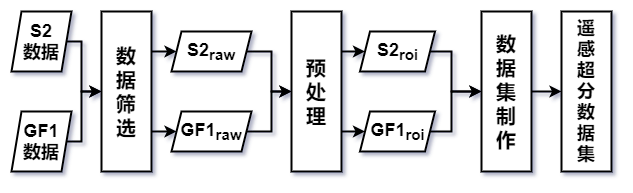
\includegraphics[width=0.9\textwidth]{pic/chap02-01.png}
    \caption{超分辨率数据集制作整体流程图}
    \label{fig:0201}
\end{figure}

对测绘院提供的高分一号数据和欧空局哨开源的兵二号数据首先进行数据筛选, 主要关注遥感数据的成像时间和覆盖范围, 选取有一定时空交集的高分一号数据文件$GF1_{raw}$和哨兵数据$S2_{raw}$文件作为超分数据集的原始数据; 对$GF1_{raw}$和$S2_{raw}$进行预处理, 包括辐射定标, 大气校正, 正射校正, 影像融合, 影像配准, 感兴趣区域裁剪, 最终得到$GF1_{roi}$和$S2_{roi}$作为超分数据集感兴趣区域(ROI); 最后对$GF1_{roi}$和$S2_{roi}$进行裁剪和直方图匹配得到高分哨兵遥感影像超分数据集$GF1S2-SRDataset$. 本章对制作遥感影像超分辨率数据集的思路和细节进行探究, 并记录实验过程中遇到一些问题. 

\subsection{遥感数据筛选}
遥感数据筛选的目的是从海量的遥感数据中, 通过遥感数据的拍摄时间, 覆盖范围与成像质量, 筛选出具有一定时空交集的遥感数据(文件)用于制作遥感影像超分辨率数据集. 其流程如图~\ref{fig:0202}~所示:

\begin{figure}[!htbp]
    \centering
    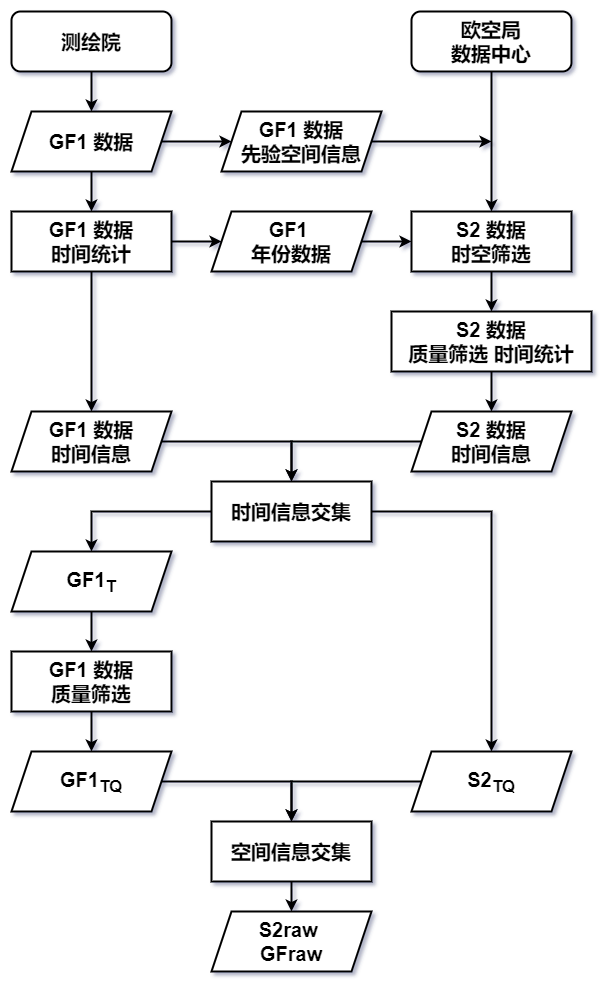
\includegraphics[height=0.60\textheight]{pic/chap02-02.png}
    \caption{遥感数据筛选流程图}
    \label{fig:0202}
\end{figure}

\href{https://scihub.copernicus.eu/dhus/#/home}{欧空局数据中心}~可以在地图中框选设置感兴趣范围, 同时也提供了卫星型号, 时间检索的按钮, 通过其网站可视化界面, 从业者可轻松从在线数据库中检索得到需要的哨兵二号影像. 此外, 点击感兴趣哨兵影像可得到对应数据的缩略图和云雾覆盖比等数据质量信息. 这为超分辨率数据集制作提供了很大的便利; 广东省国土资源测绘院提供了大量广东省高分一号遥感卫星影像, 单个高分一号数据包括全色影像和光学影像, 其占用磁盘空间较大, 由于数据格式规范, 同时基于数据安全的考虑, 在数据传输过程中进行了两次压缩, 导致解压文件的时间成本变高. 直接打开高分一号影像, 目视判别与哨兵二号影像是否有空间交集的难度也随之急剧增长. 

因此, 在数据筛选的过程中, 根据难易程度, 先筛选哨兵数据, 之后再用哨兵数据结果筛选高分数据.针对以上高分和哨兵数据信息获取的特点, 为保证数据集制作的高效率, 首先利用测绘院提供的高分一号数据的大致覆盖范围和高分一号数据文件命名统计出的年份信息, 在~\href{https://scihub.copernicus.eu/dhus/#/home}{欧空局数据中心}~进行哨兵二号数据的检索, 共有2608幅影像. 通过云雾覆盖率剔除掉质量较差无法用于数据集制作的数据, 如图~\ref{fig:0203}~所示:

\begin{figure}[!htbp]
    \centering
    \subfloat[云雾全覆盖]{\label{fig:0203a}
    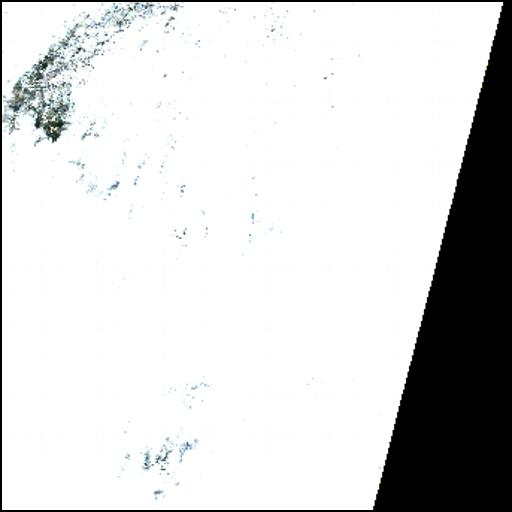
\includegraphics[width=12em]{pic/chap02-03a.jpg}}
    \quad
    \subfloat[云雾全图分布密集]{\label{fig:0203b}
    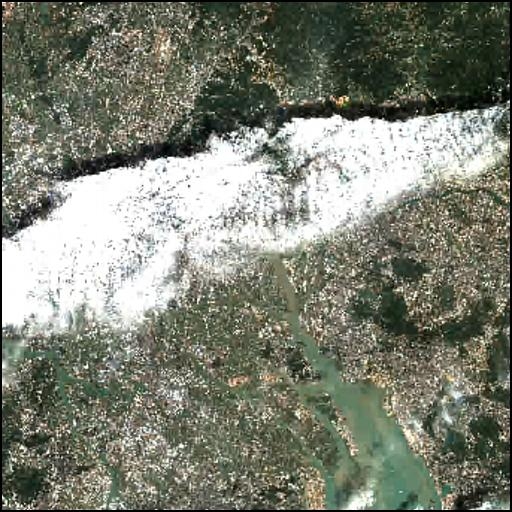
\includegraphics[width=12em]{pic/chap02-03b.jpg}}
    \caption{质量较差的哨兵二号影像}
    \label{fig:0203}
\end{figure}

在图~\ref{fig:0203a}~中, 影像的云雾覆盖率过高, 达99\%以上, 在图~\ref{fig:0203b}~中, 虽云雾覆盖没有图~\ref{fig:0203a}~严重, 但点状的云朵密集分布于影像上下侧, 为了剔除云雾影响而产生的工作量, 对数据集制作的后续步骤将是毁灭性打击. 若云雾集中分布于影像一侧或一角, 则无云雾覆盖或是云雾分布稀疏的影像部分可用于超分数据集制作, 如图~\ref{fig:0204}~所示, 其中图~\ref{fig:0204a}云雾分布在左下角, 图~\ref{fig:0204b}云雾集中分布左侧. 尽管这种数据并非理想型, 仍建议先保留, 以防后期高分哨兵时空交集数据缺失, 无法制作数据集. 

\begin{figure}[!htbp]
    \centering
    \subfloat[云雾集中分布一角]{\label{fig:0204a}
    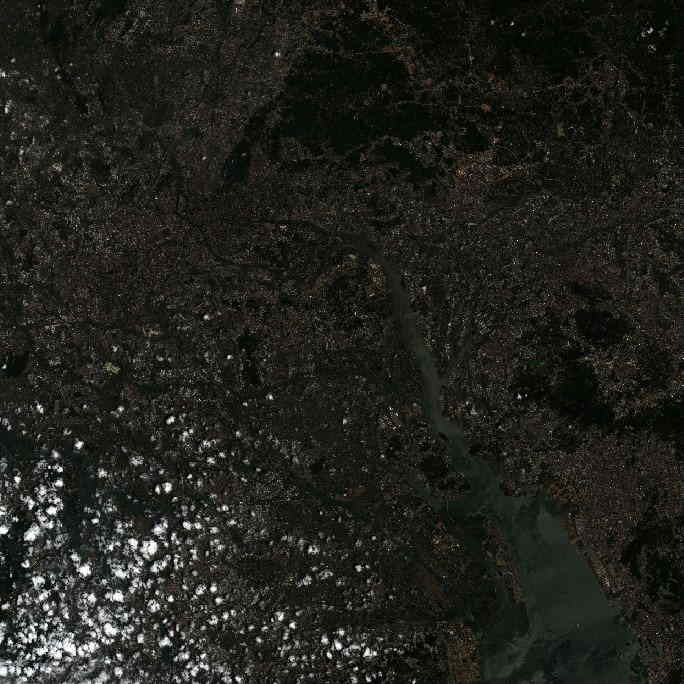
\includegraphics[width=12em]{pic/chap02-04a.jpg}}
    \quad
    \subfloat[云雾集中分布一侧]{\label{fig:0204b}
    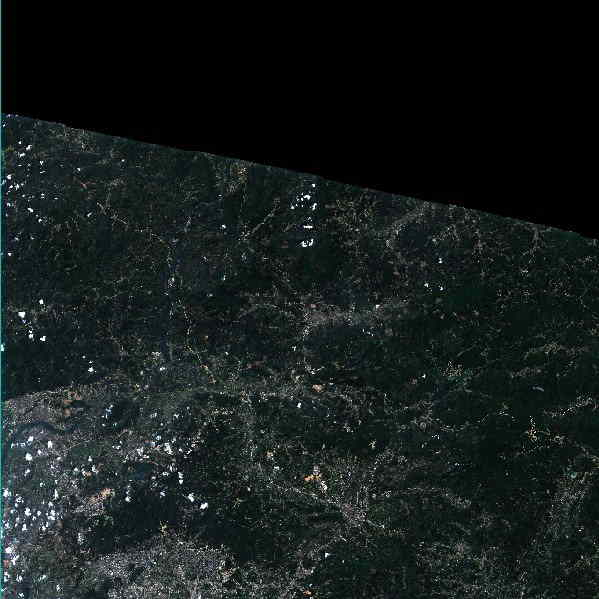
\includegraphics[width=12em]{pic/chap02-04b.jpg}}
    \caption{质量可接受的哨兵二号影像}
    \label{fig:0204}
\end{figure}

在剔除云雾覆盖率过高或是均匀分布整幅影像的数据后, 可用的哨兵影像有65幅, 成像时间在该年一至四月, 十至十二月, 与我国华南地区夏季多云多雨的热带气候相符. 由于高分一号只有该年一至七月与上一年十二月数据, 因此接下来遥感数据筛选过程中, 除去高分一号六七月数据, 哨兵二号十至十二月数据, 这为数据解压省去了很多时间成本, 提高了数据集整体制作效率.

由于轨道参数不同, 不同卫星时间周期有所差别, 无法做到在同一时刻拍摄同一地物. 每一地理实体都有其固定的空间范围和时间范围, 而不同任务对遥感影像时间分辨率要求不同~\cite{day14paper}, (本文认为)对于超分任务, 14天之内可认为影像内同一地物未发生变化. 因此, 寻求高分一号数据与可用哨兵二号数据中成像时间相差在14天内的数据, 此时得到时间交集后的高分一号数据$GF1_{T}$, 与经过时间交集影像质量合格的哨兵二号数据$S2_{TQ}$, 其中$T$代表经过时间(Time)交集, $Q$代表质量(Quality)合格.

和哨兵影像数据质量筛选相同, 逐步解压高分数据, 剔除如图~\ref{fig:0205a}~只有中心一小部分可用于数据集制作和图~\ref{fig:0205b}~云雾覆盖十分严重的影像, 得到有时间交集且质量合格可用于超分数据集制作的$GF1_{TQ}$. 鉴于高分一号影像覆盖范围相对于哨兵二号较小, 如果其影像中云雾覆盖过半, 后期整幅影像也要经过预处理, 融合等步骤, 那么使用此类高分影像制作数据集性价比较低, 因此不同于哨兵数据, 认为此影像不合格, 不做保留. 经过此步骤, 按月份得到多组待空间交集的高分哨兵数据集.

\begin{figure}[!htbp]
    \centering
    \subfloat[可用数据少]{\label{fig:0205a}
    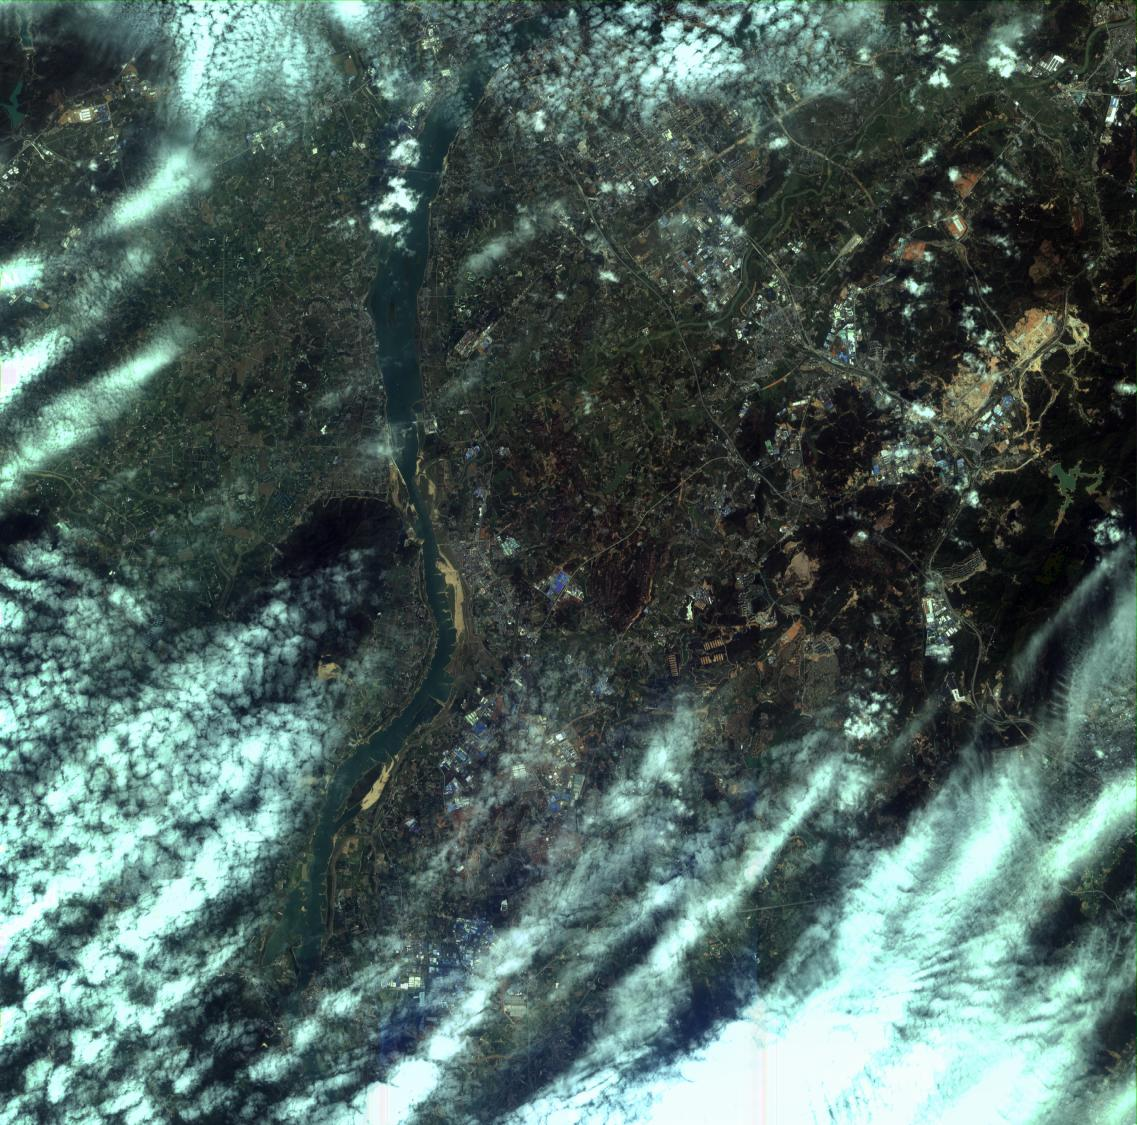
\includegraphics[width=12em]{pic/chap02-05a.jpg}}
    \quad
    \subfloat[雨雾覆盖严重]{\label{fig:0205b}
    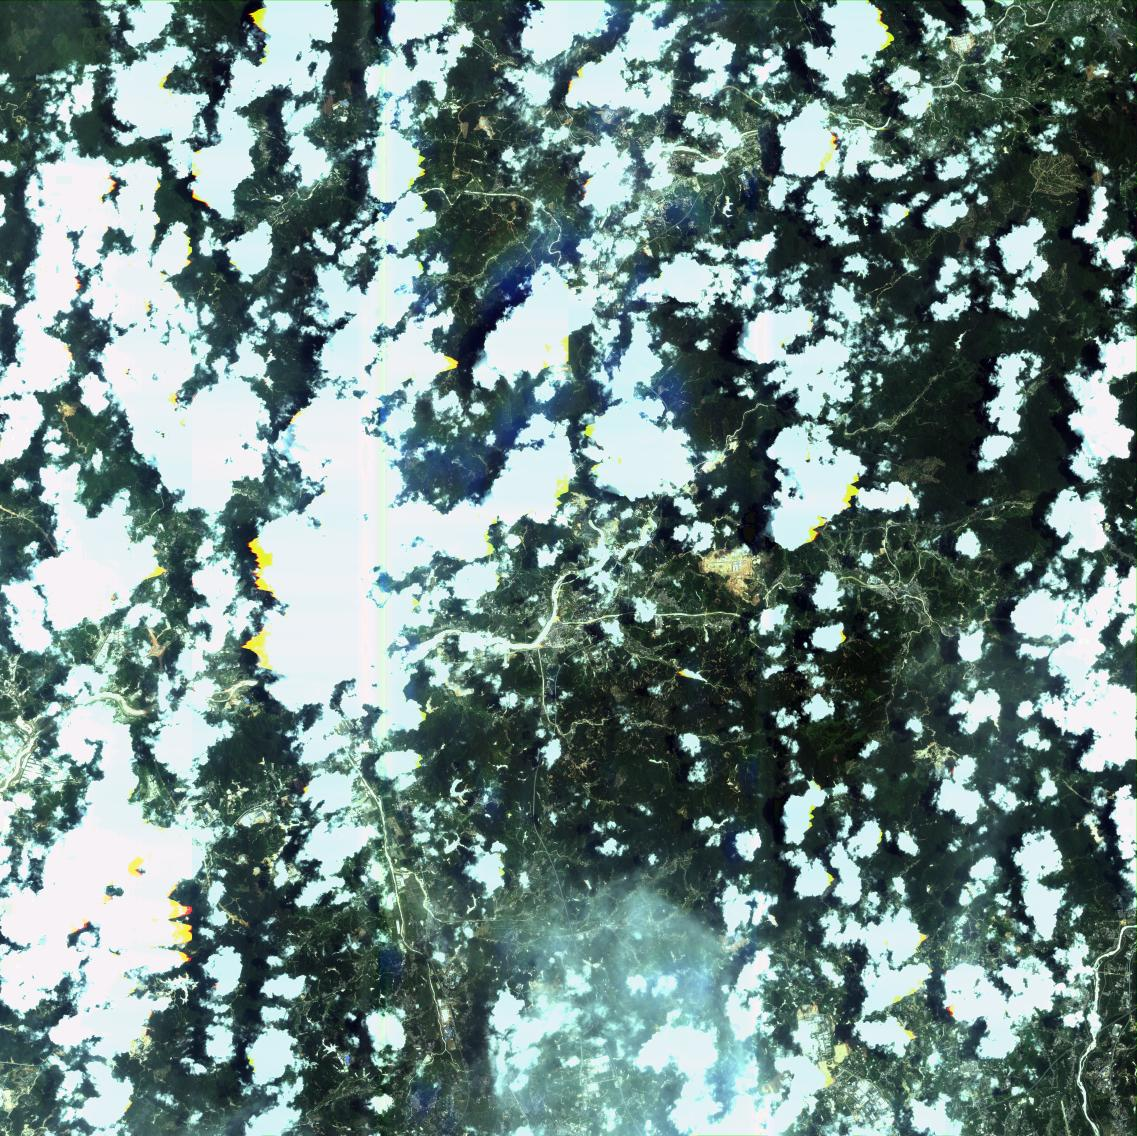
\includegraphics[width=12em]{pic/chap02-05b.jpg}}
    \caption{质量过差的高分一号影像}
    \label{fig:0205}
\end{figure}

使用ENVI软件打开每一组的高分一号影像和哨兵二号影像(具体操作可见~\ref{sec:this}~章), 通过目视判别, 确认高分影像与哨兵影像空间交集是否可用, 筛选出可用于遥感影像超分辨数据集制作的文件$GF1_{raw}$和$S2_{raw}$. 以其中一组的结果为例, 如图~\ref{fig:0208}~所示, 蓝框及有明显色差的为高分数据(todo换图):

\begin{figure}[!htbp]
    \centering
    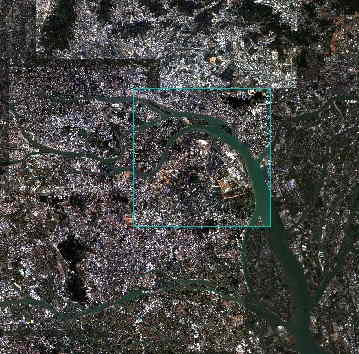
\includegraphics[height=15em]{pic/chap02-08.jpg}
    \caption{数据筛选结果}
    \label{fig:0208}
\end{figure}

\subsection{遥感影像预处理}
在遥感影像预处理的目的是对筛选好的$GF1_{raw}$和$S2_{raw}$进行预处理, 包括: 辐射定标, 大气校正, 正射校正, 影像融合, 影像配准, 影像裁剪等, 如图~\ref{fig:0206} 所示, 得到可用作遥感超分辨率数据集的$GF1_{roi}$, $S2_{roi}$. 

\begin{figure}[!htbp]
    \centering
    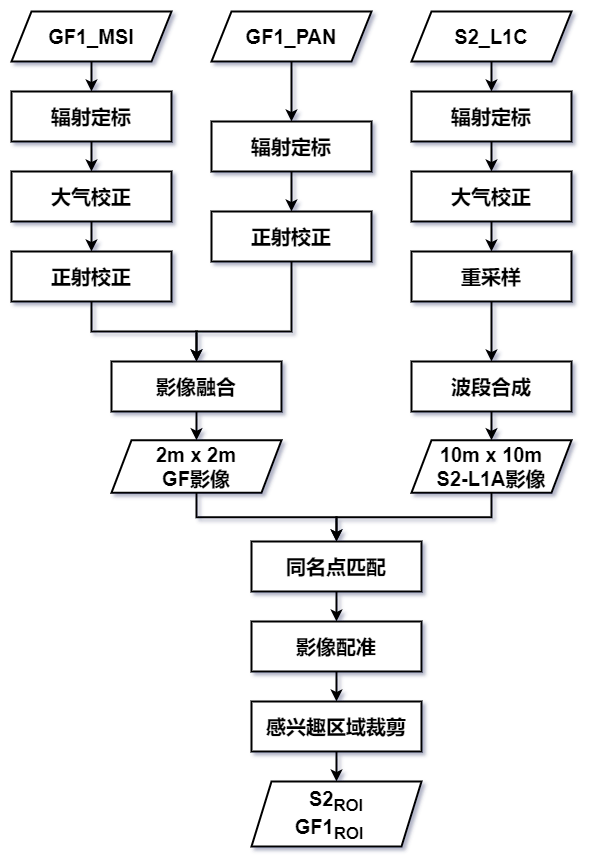
\includegraphics[height=0.70\textheight]{pic/chap02-06.png}
    \caption{遥感数据预处理流程图}
    \label{fig:0206}
\end{figure}

由于遥感影像成像过程的复杂性, 传感器接收到的电磁波能量与目标本身辐射的能量是不一致的~\cite{RSbook01}. 传感器输出的能量包含了太阳位置, 大气条件以及传感器本身性能所引起的各种失真, 这些失真不是地面目标本身的辐射, 会对之后影像使用造成影响, 必须加以校正或消除. 因此要对高分一号和哨兵二号影像进行辐射校正和几何校正.

\subsubsection{高分一号影像校正与融合}

\subsubsection*{辐射定标}
辐射定标是将传感器记录的电压或数据量化值(DN)转换为绝对辐射亮度值(辐射率), 或者转换为地表反射率, 表面温度等物理量的过程~\cite{RSbook01}. 辐射定标分为绝对定标与相对定标. 绝对定标对目标作定量描述, 得到目标的辐射绝对值; 相对定标是得出目标中某一点辐射亮度与其他点的相对值. 绝对定标要建立传感器测量的数字信号与对应的辐射能量之间的数量关系, 即定标系数. 绝对辐射定标如式~\ref{eq:02-01}~所示:

\begin{equation}
    L_{\lambda}=Gain * DN + Bias
    \label{eq:02-01}
\end{equation}

其中, $L_{\lambda}$为辐射亮度, 单位为: $w \cdot cm^{-2} \cdot \mu m^{-1} \cdot sr^{-1} $; 辐射定标参数$Gain$以及$Bias$分别为定标增益和偏移量. 不同传感器对应标定参数不同. ENVI并不支持国产遥感卫星\label{sec:this}, 需要安装~\href{http://blog.sina.com.cn/s/blog_764b1e9d0102xjbj.html#cmt_5AD807AE-3B2A6BFD-6A4E9A6B-91B-8EF}{ENVI扩展工具: 中国国产卫星支持工具}~, 才可打开高分一号影像同时获取其传感器的定标参数, 或者可在~\href{http://www.cresda.com/CN/Downloads/dbcs/index.shtml}{中国资源卫星应用中心}~中查询到定标参数, 选择手动编辑. 在ENVI5.3中, 使用``Radiometric Correction/Radiometric Calibration''工具对高分一号多光谱影像GF1MSI和全色影像GF1PAN进行辐射定标.

\subsubsection*{大气校正}
大气对阳光和来自目标的辐射产生吸收和散射. 太阳辐射经过气体分子的吸收和气溶胶粒子散射, 得到减弱, 同时部分散射信号直接或经过地物反射进入传感器, 又得到增强. 这降低了影像的反差比, 使影像可读性降低. 因此在影像配准中, 消除大气影响十分重要, 这一过程称之为大气校正. 大气校正目的是消除遥感影像中大气分子, 气溶胶的散射和吸收作用~\cite{RSbook01}. 使用ENVI5.3软件的 FLAASH 校正工具完成已辐射定标过的高分多光谱影像GF1-MSI的大气校正, 全色影像不需要大气校正.  

\subsubsection*{正射校正}
由于传感器平台自身的高度, 姿态等不稳定, 或是地球曲率, 地形等影响, 使得遥感影像出现几何变形~\cite{RSbook01}, 因此需要做几何校正来消除这些变形. 遥感影像的几何校正分为几何粗校正和几何精校正, 一般我们获取的影像数据都是经过几何粗校正. 精校正主要借助地面控制点使影像的几何位置符合某种地理坐标系统, 其中正射校正不仅能实现常规几何校正功能, 还能通过测量点的高程和DEM消除地形引起的影像几何畸变. 高分一号的L1A级数据包括了RPC(Rational Polynomial Coefficients,理多项式系数), 因此可以直接使用``Geometric Correction/Orthorectification/RPC Orthorectification Workflow''工具对经过辐射校正的GF1-MSI和GF1-PAN进行正射校正. 

\subsubsection*{影像融合}
全色影像具有较高的空间分辨率, 多光谱影像含有丰富的光谱信息, 为了能充分利用全色影像的空间特征和多光谱影像丰富的光谱特征, 需要将全色影像和多光谱影像进行融合处理. 此为得到高分辨率遥感影像的关键步骤.

经过辐射校正和几何校正后, 得到空间分辨率为8m多光谱影像GF1-MSI和空间分辨率为2m的全色影像GF1-PAN影像. 在ENVI5.3中, 可使用的影像融合方法有多种, 其中NNDiffuse方法~\cite{NNDfuse}优于其他方法, 融合结果对于色彩, 纹理和光谱信息, 均能得到很好保留. 因此使用 ``Image Sharpening/NNDiffuse Pan Sharpening''工具进行影像融合, 得到具有2m分辨率的融合影像, 如图~\ref{fig:0207}~所示:

\begin{figure}[!htbp]
    \centering
    \subfloat[融合前8m分辨率]{\label{fig:0207a}
    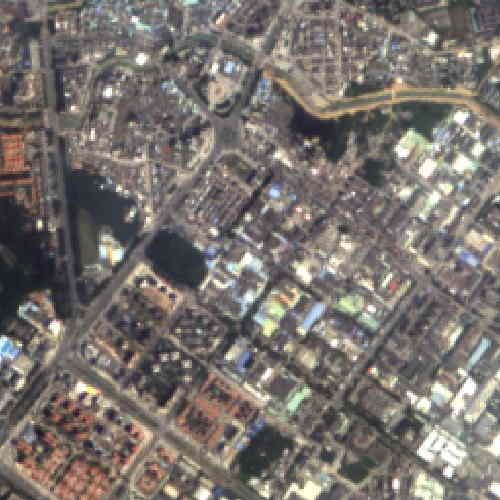
\includegraphics[width=11em]{pic/chap02-07a.jpg}}
    \quad
    \subfloat[融合后2m分辨率]{\label{fig:0207b}
    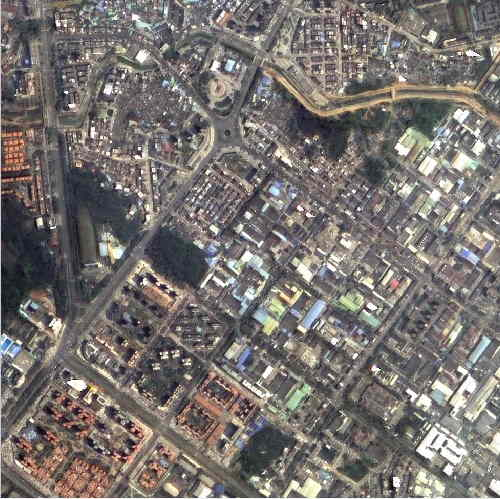
\includegraphics[width=11em]{pic/chap02-07b.jpg}}
    \caption{融合结果对比}
    \label{fig:0207}
\end{figure}

\subsubsection{哨兵二号影像校正与处理}
在~\href{https://scihub.copernicus.eu/dhus/#/home}{欧空局数据中心}~下载的L1C级别的哨兵二号影像已经做过了正射校正~\cite{S2handbook}, 哨兵二号影像辐射校正方法与高分一号大致相同, 直接使用欧空局提供的插件~\href{http://step.esa.int/main/snap-supported-plugins/sen2cor/}{Sen2Cor}~即可轻松完成哨兵二号影像的预处理, 得到L1A级别的哨兵二号影像. 

对哨兵二号影像的后续处理需要在ENVI软件中, 而哨兵二号影像文件只能被欧空局开发的遥感影像处理软件SNAP打开, 因此需要转换文件的格式. 由于哨兵二号各波段分辨率不同~\cite{S2handbook}, 无法直接转换为ENVI格式文件, 需要在SNAP中使用 ``raster/geometric operations/resampling''工具重采样, 之后转换为ENVI格式文件; 在ENVI中打开Band2(Blue), Band3(Green), Band4(Red), 使用 ``Raster Management/Layer Stacking''工具波段合成, 得到可在ENVI中打开的哨兵二号光学遥感影像. 

\subsubsection{影像配准与裁剪}
超分数据集中高低分辨率影像应严格为同一场景, 由于遥感影像不同源, 经过辐射校正和几何校正的高分一号影像和哨兵二号影像, 同一地物在空间上仍有一定偏差, 如图~\ref{fig:0209}~所示, 十字红线交叉点代表同一经纬度地物, 可明显发现, GF1 影像中对应浅蓝色厂房角点在 S2 影像中向左有偏移(todo换图). 在后续的步骤中, 根据经纬度划定感兴趣区域, 这会造成裁剪出的高分一号影像与哨兵二号影像并未严格包含相同场景, 因此必须对高分和哨兵影像进行影像配准. 

\begin{figure}[!htbp]
    \centering
    \subfloat[GF1]{\label{fig:0209a}
    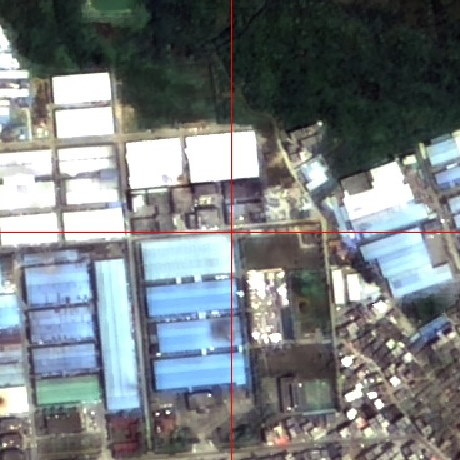
\includegraphics[width=10em]{pic/chap02-09a.jpg}}
    \quad
    \subfloat[S2]{\label{fig:0209b}
    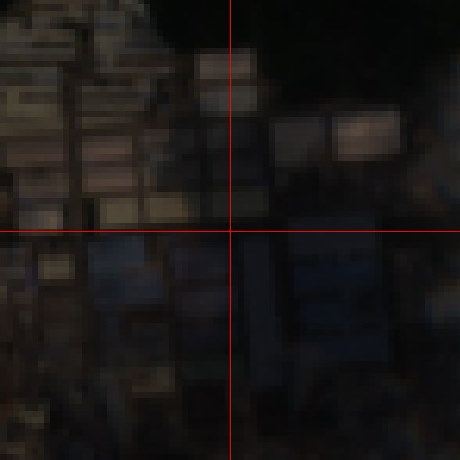
\includegraphics[width=10em]{pic/chap02-09b.jpg}}
    \caption{空间偏差结果}
    \label{fig:0209}
\end{figure}

图像配准是将位于不同坐标系下同一场景的二幅或多幅图像, 寻找一种特定的最优几何变换, 将两幅或多幅图像变换到同一坐标系的过程~\cite{ImageReg}. 其基本步骤包括: 特征检测, 特征匹配, 几何变换模型参数估计, 配准图像重采样与变换四个步骤. 遥感影像配准在应用层面较为成熟, 在ENVI的``Georectification Tools/Image Registration''工具中, 已集成Forstner, Moravec, Harris特征点检测算法, 通过调整匹配窗口大小和搜索窗口大小进行同名点匹配, 使用匹配分数和同名点最小允许误差对匹配到的同名点进行筛选, 得到质量较好的同名点, 据其估计几何变换模型最佳参数, 并重采样匹配影像进行变换配准, 得到影像配准后的影像. 实验用高分影像作为配准影像, 哨兵影像作为待配准影像.  

同名点的分布及数量决定了图像配准的质量. 在同名点分布均匀且密集的区域内, 图像配准效果比较好, 此种区域比较适合作为感兴趣区域进行裁剪, 如图~\ref{fig:0210}~所示, 图~\ref{fig:0210a}~中粉色表示高分影像中同名点, 图~\ref{fig:0210b}~中彩色方块代表不同感兴趣区域. 借助于ENVI优秀的软件设计与可视化界面, 对于同名点分布稀疏的地方, 可以手动添加同名点. 为了后续批量处理方便, 感兴趣区域影像裁剪应当裁剪为水平矩形. 

\begin{figure}[!htbp]
    \centering
    \subfloat[同名点检测结果]{\label{fig:0210a}
    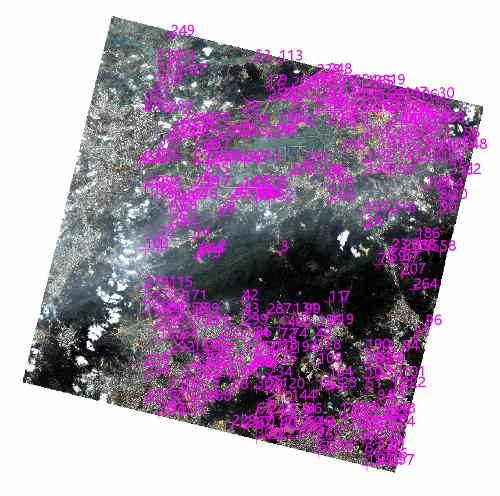
\includegraphics[width=12em]{pic/chap02-10a.jpg}}
    \quad
    \subfloat[影像裁剪]{\label{fig:0210b}
    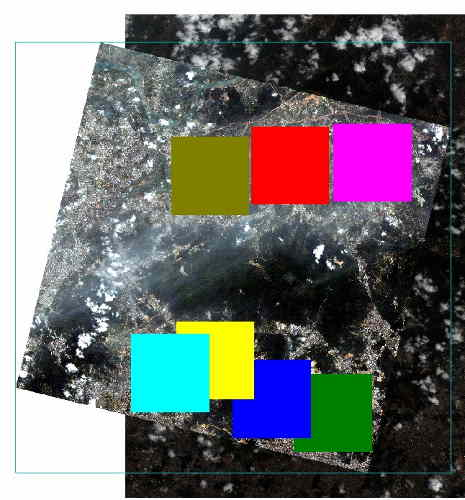
\includegraphics[width=12em]{pic/chap02-10b.jpg}}
    \caption{同名点检测结果与影像裁剪}
    \label{fig:0210}
\end{figure}

每一组$GF1_{raw}$和$S2_{raw}$经过辐射校正, 正射校正等处理后,ENVI导出裁剪的感兴趣区域, 得到对应png格式的$GF1_{roi}$和$S2_{roi}$. 

\subsection{遥感超分辨率数据集制作}
批量裁剪; 人工除去差异较大, 云雾覆盖严重; 进行直方图归一化原因, 给表格说明高分一号MSI波段差异和哨兵二号MSI差异

\subsection{本章小结}
